\documentclass{article}
\usepackage[utf8]{inputenc}
\usepackage{geometry}
 \geometry{
 a4paper,
 total={170mm,257mm},
 left=20mm,
 top=20mm,
 }
\usepackage{tikz}\usetikzlibrary{automata, positioning, arrows}

\title{ COMP 330 Winter 2021 \\ Assignment 3}
\author{Belle Pan 260839939}
\date{18th February 2021}

\usepackage{natbib}
\usepackage{graphicx}

\begin{document}

\maketitle

\noindent \textbf{Solution 1. 
\\Are the following statements true or false? Prove your answer in each case, but the proof need only be a simple example or a couple of lines of explanation. We have some fixed alphabet \(\Sigma\) with at least two letters. In the following \(A\) and \(B\) stand for languages, i.e. subsets of \(\Sigma^*\)
\begin{itemize}
    \item If \(A\) is regular and \(A \subseteq B\) then \(B\) must be regular.
    \item If \(A\) is regular and \(AB\) are both regular then \(B\) must be regular.
    \item If \(\{A_i|i\in \N\}\) is an infinite family of regular sets then \(\bigcup\limits_{i=1}^{\infty} A_{i}\) is regular.
    \item If \(A\) is not regular it cannot have a regular subset.
\end{itemize}
}
\\
\\\noindent The following are the true/false value with the reasoning for each respective sub-question:
\begin{itemize}
    \item False. We know that \(A\) is regular because all finite sets are regular; however, there is no information stating that \(B\) is a finite set! Therefore, we cannot simply say that \(B\) is regular.
    \item False. If \(A\) is the finite set \(\Sigma^*\) and \(B\) is irregular, \(AB\) is still regular as \(AB = \Sigma^*\). Therefore, \(B\) is not always regular in this case.
    \item False. \(\bigcup\limits_{i=1}^{\infty} A_{i}\) is an infinite set and is therefore not regular.
    \item False. All finite sets are regular, so a finite subset of \(A\) must also be regular.
\end{itemize}
\\
\\


\noindent \textbf{Solution 2. 
\\Show that the following language is not regular using the pumping lemma : \(\{a^n b^{2n}|n>0\}\).}
\\
\\\noindent Below is a proof using the demon - angel strategy of showing the pumping lemma:
\begin{enumerate}
    \item The demon picks a number p.
    \item The angel picks the word \(a^p b a^{2p}\).
    \item The demon is forced to pick a \(y\) value that is made of exclusively \(a\)'s due to the constraints \(|xy|\leq p\) and \(|y|>0\). Suppose that \(y=a^k\) such that \(0<k\leq p\).
    \item The angel chooses \(i=2\) such that the new word becomes \(a^{p+k} b a^{2p}\). This word is not in the language as \(p+k \neq 2\times p\).
\end{enumerate}
Thus, by the pumping lemma, \(\{a^n b^{2n}|n>0\}\) is indeed not a regular language.
\\
\\


\noindent \textbf{Solution 3. 
\\Show that the language \(F=\{a^ib^jc^k|i,j,k \geq 0\) and if \(i=1\) then \(j=k\}\) is not regular. Show, however, that it satisfies the statement of the pumping lemma as shown in class, i.e. there is a \(p\) such that all three conditions for the pumping lemma are met. Explain why this does not contradict the pumping lemma.}
\\
\\\noindent We start with showing that \(F\) is not regular:
\begin{itemize}
    \item First, we know that we cannot use the pumping lemma, as it is clear by the question that \(F\) satisfies the pumping lemma.
    \item We must use the closure properties of regular languages to prove that \(F\) is not regular, particularly the property that the intersect (\(\cap\)) of two regular languages produces a regular language.
    \item We define a language \(F' = \{a b^j c^k | j, k \geq 0\}\) such that \(F \cap F' = \{a b^n c^n\ | n \geq 0\}\). This is clearly NOT a regular language, as a DFA cannot count the number of occurrences of \(b\) and \(c\) and ensure that they are equal. 
    \item Therefore, \(F\) is NOT a regular language!
\end{itemize}
\noindent Next, we must show that \(F\) satisfies the pumping lemma:
\begin{itemize}
    \item It is important to note that the pumping lemma states that all regular languages are pump-able, but it does NOT state that a pump-able language is regular (i.e. all regular languages \(\Longrightarrow\) pump-able, and the converse is not true). Thus, even if \(F\) satisfies the pumping lemma, it does not necessarily mean that \(F\) is regular!
    \item As we will be proving that \(F\) satisfies the pumping lemma, we do not use the negation method that is often used to prove that a language is not regular, i.e. in this case the angel will begin the game and choose the \(p\) value.
    \begin{itemize}
        \item The angel chooses \(p=2\).
        \item The demon chooses \(w = a^m b^j c^k\).
        \begin{itemize}
            \item When \(m=0\), \(w=b^j c^k\).
            \begin{itemize}
                \item The angel chooses \(y=b\) if the word begins with \(b\), OR the angel chooses \(y=c\) if the word begins with \(c\); these follow the restraints of \(|xy|\leq p\) and \(|y| \leq p\) when \(x=\epsilon\).
                \item The demon chooses an \(i\) value, such that the new word is either \(b^i b^{j-1} c^k\) if \(y=b\), OR \(c^i c^{k-1}\) if \(y=c\). These two words are clearly in \(F\), thus \(F\) satisfies the pumping lemma when \(m=0\).
            \end{itemize}
            \item When \(m=1\), \(w=a b^j c^k\).
            \begin{itemize}
                \item The angel chooses \(y=a\); this follows the restraints of \(|xy|\leq p\) and \(|y| \leq p\) when \(x=\epsilon\).
                \item The demon chooses an \(i\) value such that the new word is \(a^i b^j c^k\); this is clearly in \(F\), and thus \(F\) satisfies the pumping lemma when \(m=1\).
            \end{itemize}
            \item When \(m=2\), \(w=a^2 b^j c^k\).
            \begin{itemize}
                \item The angel chooses \(y=a^2\); this follows the restraints of \(|xy|\leq p\) and \(|y| \leq p\) when \(x=\epsilon\). We choose \(y=a^2\) because words in the form of \(a b^j c^k\) may not necessarily be in \(F\).
                \item The demon chooses an \(i\) value such that the new word is \(a^{2i} b^j c^k\); this is clearly in \(F\), and thus \(F\) satisfies the pumping lemma when \(m=2\).
            \end{itemize}
            \item When \(m> 2\), \(w=a^m b^j c^k\).
            \begin{itemize}
                \item The angel chooses \(y=a\); this follows the restraints of \(|xy|\leq p\) and \(|y| \leq p\) when \(x=\epsilon\).
                \item The demon chooses an \(i\) value such that the new word is \(a^i a^{m-1} b^j c^k\); this is clearly in \(F\) as \(m-1>1\), and thus \(F\) satisfies the pumping lemma when \(m> 2\).
            \end{itemize}
        \end{itemize}
    \end{itemize}
    \item Therefore, given the above proof, \(F\) satisfies the pumping lemma. \(F\), despite being a non-regular language, satisfies the pumping lemma because the lemma only states that all regular languages are pump-able, NOT that all pump-able languages are regular!
\end{itemize}
\\
\\

\newpage
\noindent \textbf{Solution 4. 
\\Let \(D\) be the language of words \(w\) over the alphabet \(\{a,b\}\) such that \(w\) has an even number of \(a\)'s and an odd number of \(b\)'s and does not contain the substring \(ab\). By this last statement, it is meant that one can never have an \(a\) followed by a \(b\).
\begin{enumerate}
    \item Give a DFA with only five states, including any dead states, that recognizes \(D\).
    \item Give a regular expression for this language.
\end{enumerate}
}
\begin{figure} [ht]
   \centering
    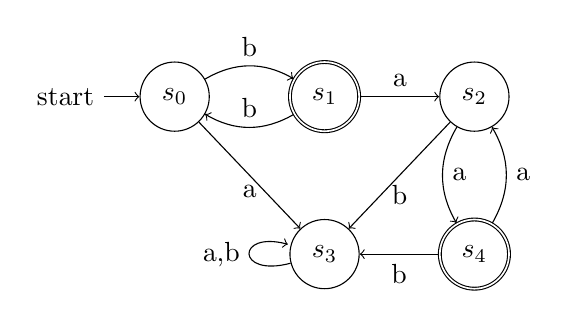
\begin{tikzpicture}
        \node[state,initial](s_0) {$s_0$};
        \node[state, accepting] (s_1) [right=of s_0] {$s_1$};
        \node[state] (s_2) [right=of s_1] {$s_2$};
        \node[state] (s_3) [below of= s_1, yshift=-1cm] {$s_3$};
        \node[state, accepting] (s_4) [below of= s_2, yshift=-1cm] {$s_4$};
        \path[->] 
                (s_0) edge [bend left] node [above] {b} (s_1)
                    edge node [below] {a} (s_3)
                (s_1) edge node [above] {a} (s_2)
                    edge [bend left] node [above] {b} (s_0)
                (s_2) edge node [below] {b} (s_3)
                    edge [bend right] node [right] {a} (s_4)
                (s_3) edge [loop left] node {a,b} ()
                (s_4) edge [bend right] node [right] {a} (s_2)
                    edge node [below] {b} (s_3);
    \end{tikzpicture}
    \caption{DFA accepting the set of all words in \(D\).}
    \label{fig:my_label}
\end{figure}
\noindent The regular expression for \(D\) is \(b(bb)^*(aa)^*\).
\\\\

\noindent \textbf{Solution 5. 
\\Consider the language  \(L = \{a^n b^m | n\neq m\}\); as seen in class, this is not regular. Recall the definition of the equivalence \(\equiv_L\) which we used in the proof of the Myhill-Nerode theorem; we used the notation \(R_L\) in the notes but it means the same thing as \(\equiv_L\). Since this language is not regular \(\equiv_L\) cannot have finitely many equivalence classes. Exhibit explicitly, infinitely many distinct equivalence classes of \(\equiv_L\).}

\\
\\
\\
\noindent 
\begin{itemize}
    \item We must first show that for two strings \(x \in L\) and \(y \in L\) such that \(x \not \equiv_L y\), there exists a string \(z\) such that \(xz \notin L\) and \(yz\in L\) or vice versa.
    \begin{itemize}
        \item Consider the two strings \(a^j\) and \(a^k\): we first claim that \(a^j \not\equiv_L a^k\) where \(j\neq k\).
        \item Then, we find a string \(z\) such that \(a^j z \notin L\) and \(a^k z\in L\).
        \item Now, we state that \(z = b^j\), which yields us \(a^j b^j\), which is clearly \(\notin L\), and \(a^k b^j\) which is clearly \( \in L\).
    \end{itemize}
    \item  Then, we need to show that there are infinitely many distinct equivalence classes.
    \begin{itemize}
        \item There is clearly an infinite number of equivalence classes as the equivalence classes of \(a^k\) are different for every value of \(k\), and there are infinitely many values of \(k\).
    \end{itemize}
    \item Therefore, there are an infinite number of equivalence classes of \(\equiv_L\).
\end{itemize}
\\\noindent 






\end{document}
